% ============================================================================
% Roadmap section-divider: HYBRID of last semester's arcade map.
%   * original cartridge art (img/roadmap/*.png, full-res from w3_rl.pptx)
%   * arrows + why-ladder bubbles redrawn natively in TikZ + Libertinus
%   * a "you are here" spotlight: current ride lit, the rest dimmed
%
% Layout follows the DECK's order, so the spotlight marches along the U-path as
% the lecture advances:  MDP -> Bandit -> Bellman -> Darts -> SARSA.
%
%   \roadmap            overview: every ride lit, the full why-ladder
%   \roadmapmdp \roadmapbellman \roadmapsarsa \roadmapbandit \roadmapdarts
% ============================================================================
\usetikzlibrary{shadows.blur}
\definecolor{spot}{HTML}{F59E0B}   % bright amber glow for the current ride

% --- one cartridge: #1 file  #2 x  #3 y  #4 lit(1)/dim(0) ---
\newcommand{\rmcard}[4]{%
  \ifnum#4=1
    \node[inner sep=0pt, draw=spot, line width=2.8pt, rounded corners=2.5pt]
      at (#2,#3) {\includegraphics[height=3.15cm]{img/roadmap/#1}};%
  \else
    \begin{scope}[transparency group, opacity=0.26]
      \node[inner sep=0pt] at (#2,#3) {\includegraphics[height=2.95cm]{img/roadmap/#1}};%
    \end{scope}
  \fi
}
% --- a bubble: #1 x  #2 y  #3 width(cm)  #4 fill  #5 textcolor  #6 text ---
\newcommand{\rmbubble}[6]{%
  \node[fill=#4, text=#5, rounded corners=3pt, align=center, font=\scriptsize,
        inner sep=4pt, text width=#3cm] at (#1,#2) {#6};%
}

% string constants for \ifx comparisons
\def\rmall{all}\def\rmmdp{mdp}\def\rmbel{bellman}\def\rmsar{sarsa}\def\rmban{bandit}\def\rmdar{darts}

% layout: cards on a U-path in deck order, why-ladder on the right
\newcommand{\rmscene}[1]{% #1 = current key (or "all")
  \begin{frame}[plain]
  % The 16cm bounding box is wider than a plain frame's \textwidth (398.34pt);
  % center it on the paper via \makebox so the layout is fixed and no overfull
  % \hbox is reported (a bare \centering would overflow by 56.9pt).
  \noindent\makebox[\textwidth][c]{%
  \begin{tikzpicture}
    \useasboundingbox (0,0) rectangle (16,9);
    \node[opacity=0.16, inner sep=0pt] at (5.6,4.5) {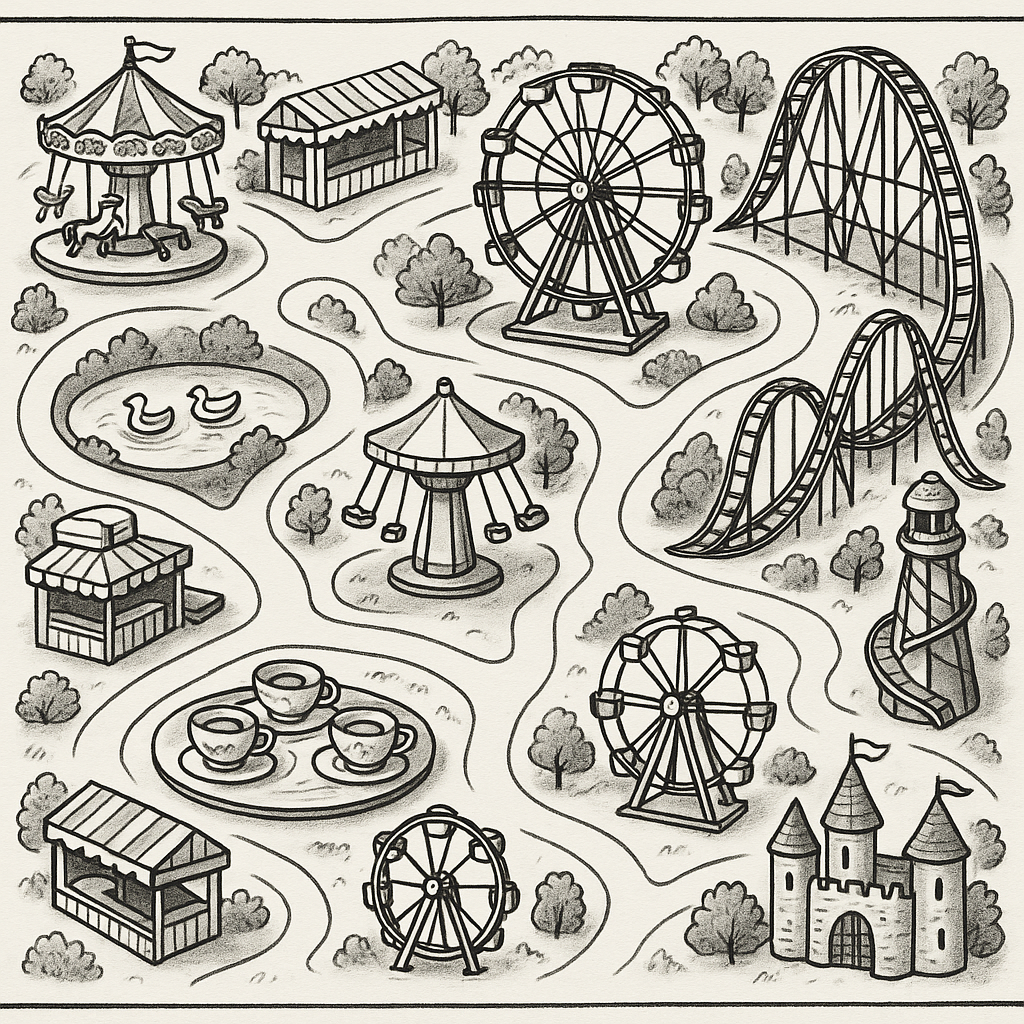
\includegraphics[height=9.2cm]{img/roadmap/park}};
    \def\cur{#1}
    \rmcard{mdp-maze}{2.4}{6.2}{\ifx\cur\rmmdp 1\else\ifx\cur\rmall 1\else0\fi\fi}
    \rmcard{bandit-arcade}{5.4}{6.2}{\ifx\cur\rmban 1\else\ifx\cur\rmall 1\else0\fi\fi}
    \rmcard{bellman-house}{8.4}{6.2}{\ifx\cur\rmbel 1\else\ifx\cur\rmall 1\else0\fi\fi}
    \rmcard{darts-dark}{8.4}{2.5}{\ifx\cur\rmdar 1\else\ifx\cur\rmall 1\else0\fi\fi}
    \rmcard{sarsa-maze}{5.2}{2.5}{\ifx\cur\rmsar 1\else\ifx\cur\rmall 1\else0\fi\fi}
    % path arrows (deck order: MDP -> Bandit -> Bellman -> Darts -> SARSA).
    % Drawn AFTER the cards so they sit on top. darts-dark.png is square (1024x1024)
    % vs the 2:3 cards, so the lit Darts card is ~3.15cm wide; the two bottom-leg
    % arrows are routed into the real gaps it leaves (down-leg shifted off the
    % "Bellman's house" label, left-leg into the SARSA<->Darts gap).
    \begin{scope}[draw=accent!75, line width=3pt, -{Stealth[length=4mm]}, opacity=0.9]
      \draw (3.55,6.2) -- (4.25,6.2);   % MDP -> Bandit
      \draw (6.55,6.2) -- (7.25,6.2);   % Bandit -> Bellman
      \draw (7.65,4.55) -- (7.65,4.18); % Bellman -> Darts (down, clear of the label)
      \draw (6.78,2.5) -- (6.42,2.5);   % Darts -> SARSA (left, in the real gap)
    \end{scope}
    \begin{scope}[font=\scriptsize\bfseries, text=black!70]
      \node at (2.4,4.35) {MDP maze}; \node at (5.4,4.35) {bandit arcade};
      \node at (8.4,4.35) {Bellman's house}; \node at (8.4,0.6) {darts in the dark};
      \node at (5.2,0.6) {SARSA maze};
    \end{scope}
    \ifx\cur\rmall
      \node[font=\large\bfseries, text=accent] at (12.5,8.55) {The plan};
      \rmbubble{12.5}{7.55}{4.2}{accent}{white}{How do we pick the best call?}
      \rmbubble{12.5}{6.5}{3.9}{good!18!white}{black!80}{the one with the largest long-run reward}
      \rmbubble{12.5}{5.35}{4.2}{accent}{white}{How do we know that reward?}
      \rmbubble{12.5}{4.3}{3.9}{good!18!white}{black!80}{the Bellman equation gives $Q^\star(s,a)$}
      \rmbubble{12.5}{3.15}{4.2}{accent}{white}{And when the odds are hidden?}
      \rmbubble{12.5}{2.1}{3.9}{good!18!white}{black!80}{learn it from experience: SARSA}
    \else
      \node[font=\large\bfseries, text=spot, anchor=north] at (12.5,8.4) {you are here};
      \rmbubble{12.5}{6.6}{4.4}{accent}{white}{\rmq}
      \rmbubble{12.5}{4.7}{4.2}{good!18!white}{black!80}{\rma}
    \fi
  \end{tikzpicture}}
  \end{frame}
}

\newcommand{\roadmap}{\def\rmq{}\def\rma{}\rmscene{all}}
\newcommand{\roadmapmdp}{%
  \def\rmq{What are we deciding, and against what?}%
  \def\rma{one call a week (run, service, replace) in a world that answers at random: a Markov decision process}%
  \rmscene{mdp}}
\newcommand{\roadmapbellman}{%
  \def\rmq{Which call wins in the long run?}%
  \def\rma{the one with the highest cumulative reward; the Bellman equation pins down its value $Q^\star(s,a)$}%
  \rmscene{bellman}}
\newcommand{\roadmapsarsa}{%
  \def\rmq{What if nobody hands us the odds?}%
  \def\rma{read the logbook: after each lived week, nudge one cell toward what it actually paid}%
  \rmscene{sarsa}}
\newcommand{\roadmapbandit}{%
  \def\rmq{Which call do we try while still learning?}%
  \def\rma{mostly the best one so far, but explore now and then, or you never learn what you skipped}%
  \rmscene{bandit}}
\newcommand{\roadmapdarts}{%
  \def\rmq{Why does nudging ever settle down?}%
  \def\rma{it is a running average of noisy evidence; Robbins and Monro proved small shrinking steps find the truth}%
  \rmscene{darts}}
